\documentclass[aspectratio=169]{beamer}

% Font setup - Montserrat
\usepackage[defaultfam,tabular,lining]{montserrat} %% Option 'defaultfam'
%% only if the base font of the document is to be sans serif
\usepackage[T1]{fontenc}
\renewcommand*\oldstylenums[1]{{\fontfamily{Montserrat-TOsF}\selectfont #1}}

% Required packages
\usepackage{xcolor}
\usepackage{tikz}
\usetikzlibrary{shapes,backgrounds,positioning,calc}

% Color definitions - Replace with your desired colors
\definecolor{primaryColor}{HTML}{334A5C}
\definecolor{backgroundColor}{HTML}{E6EAED}  
\definecolor{accentColor}{HTML}{7E8F9A}       
\definecolor{secondaryColor}{HTML}{D1DBDD} 

% Beamer theme customization
\usetheme{default}
\usecolortheme{default}

% Set main colors
\setbeamercolor{normal text}{fg=primaryColor, bg=backgroundColor}
\setbeamercolor{structure}{fg=primaryColor}
\setbeamercolor{title}{fg=primaryColor}
\setbeamercolor{frametitle}{fg=primaryColor, bg=backgroundColor}
\setbeamercolor{block title}{fg=backgroundColor, bg=accentColor}
\setbeamercolor{block body}{fg=primaryColor, bg=backgroundColor}
\setbeamercolor{item}{fg=accentColor}
\setbeamercolor{enumerate item}{fg=accentColor}

% Remove navigation symbols
\setbeamertemplate{navigation symbols}{}

% Customize frame title
\setbeamertemplate{frametitle}{
    \vspace{1em}
    \insertframetitle
    \vspace{0.5em}
}


\tikzset{
    person/.style args={#1:#2:#3}{
        minimum size=4cm, 
        path picture={
            \begin{scope}
                \clip (0, 0) circle (9mm);
                \node at (path picture bounding box.center) {
                    \includegraphics[width=18mm]{#1}
                };
            \end{scope}
            \draw[backgroundColor, line width=1.5pt] (10mm, 0) arc (0:-250:10mm);
            \node[primaryColor] at (0, -1.3) {\itshape \footnotesize #2};
            \node[primaryColor] at (0, -1.6) {\itshape \footnotesize #3};
        },
    }
}


\begin{document}

{
\usebackgroundtemplate{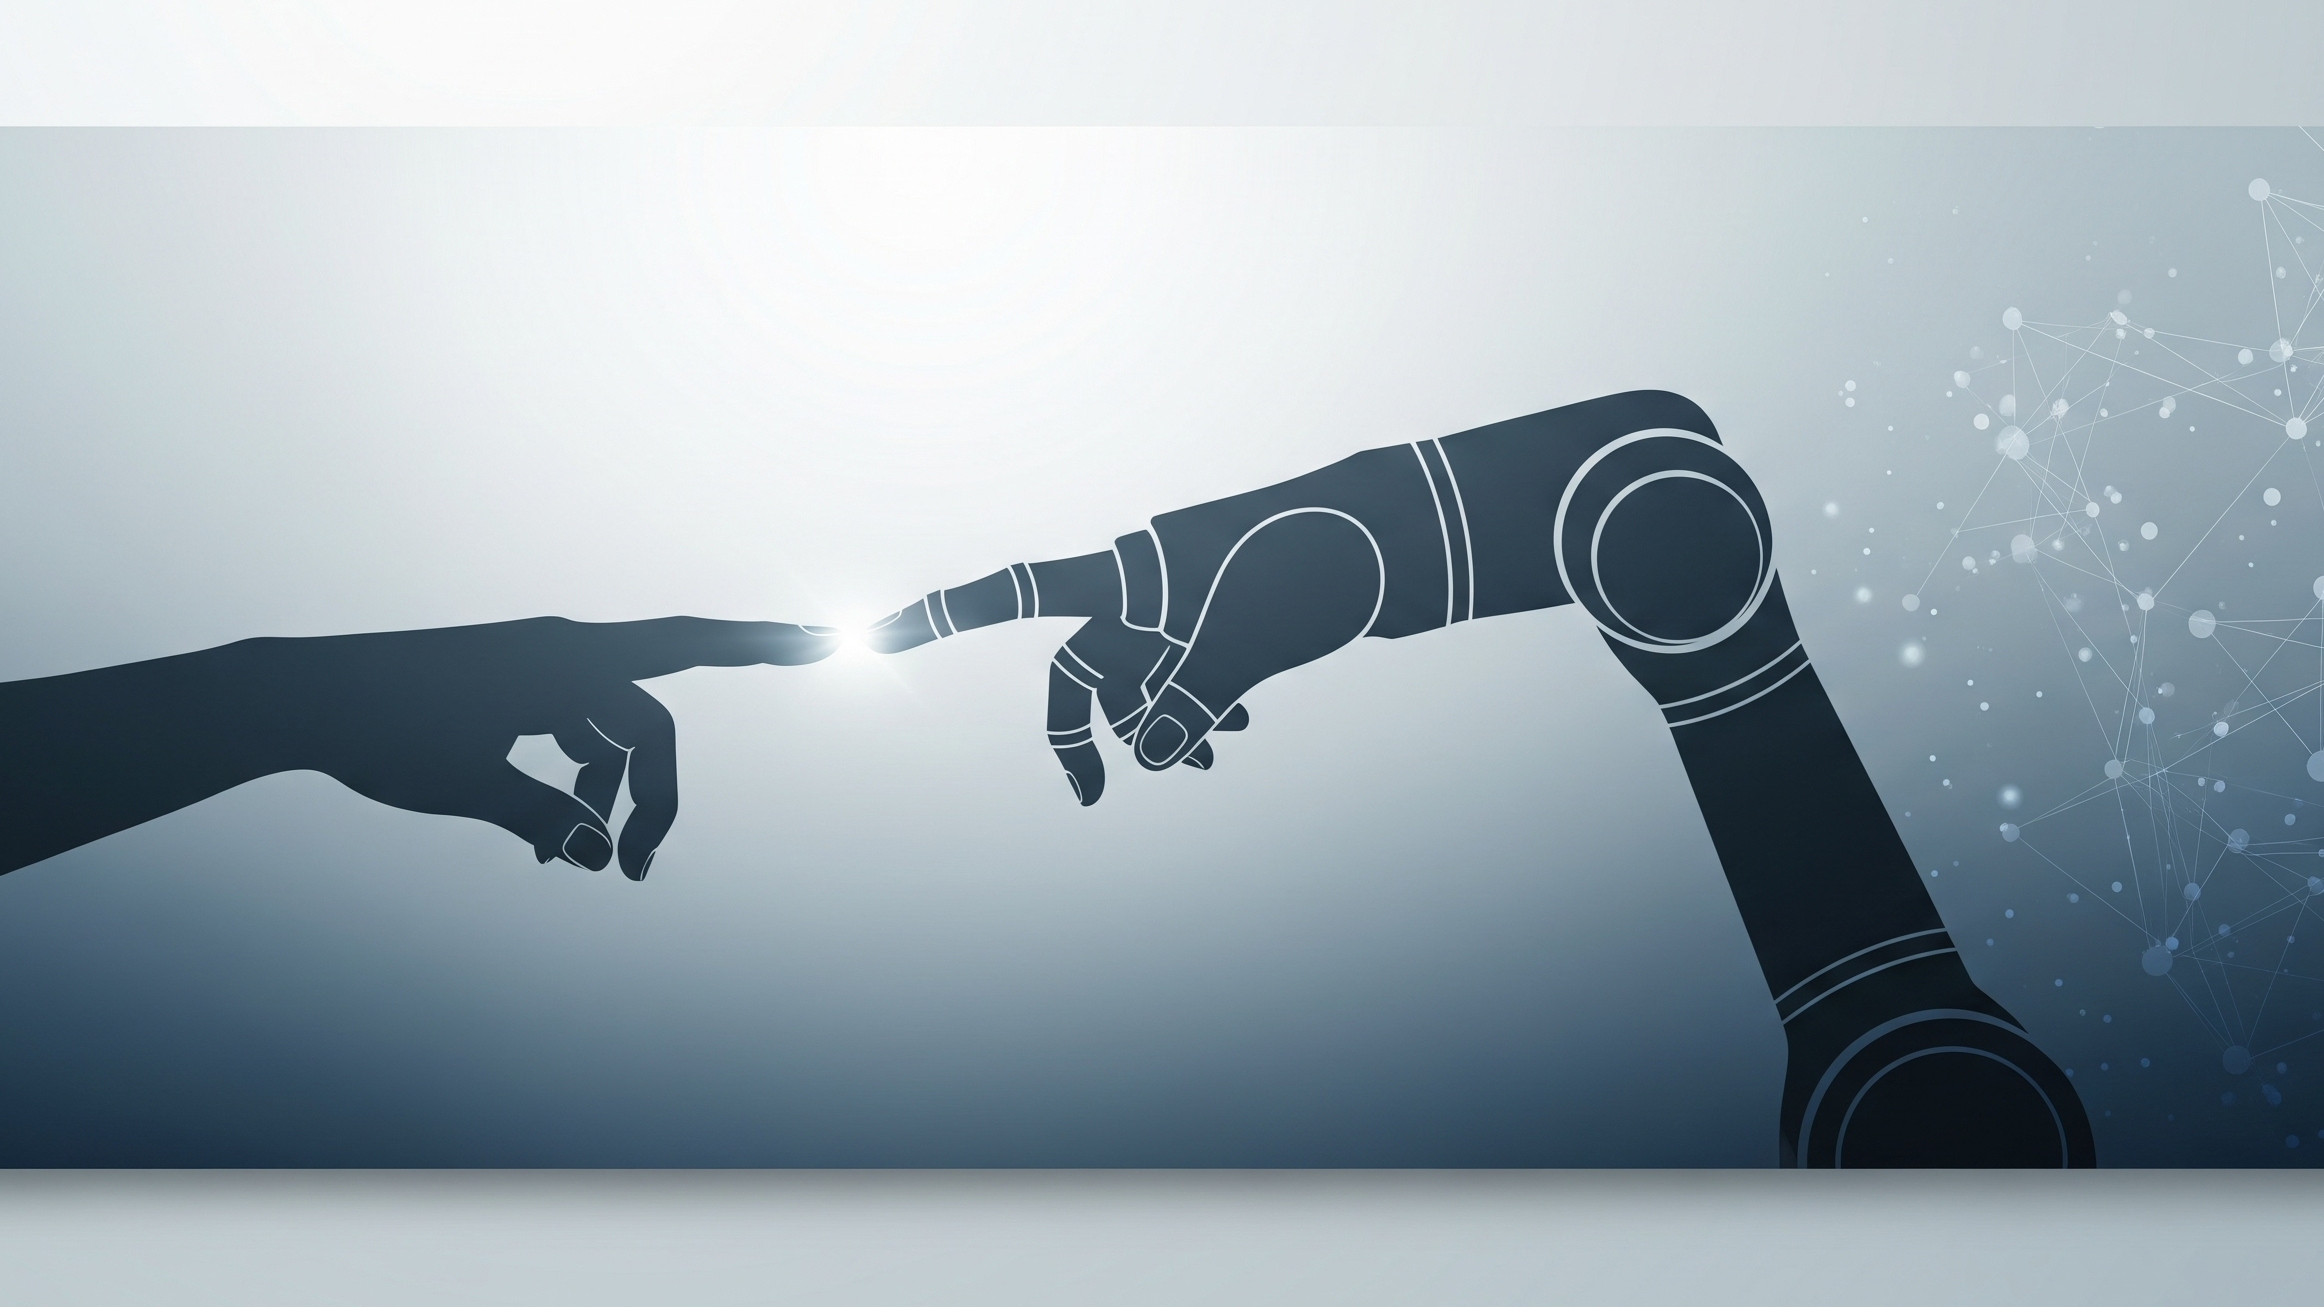
\includegraphics[width=\paperwidth]{background.png}}
\begin{frame}[plain]
    \begin{tikzpicture}[remember picture,overlay]
        \node[below right, text=primaryColor, xshift=0.3cm, yshift=-0.25cm] (WS) at (current page.north west) {Workshop ad \textit{I-RIM 3D 2025}};
        \node[primaryColor, below right, yshift=-0.1cm] (TITLE1) at (WS.south west) {\huge \textbf{Industry 5.0:}};
        \node[primaryColor, below right, yshift=1mm] (TITLE2) at (TITLE1.south west) {\Large \textbf{Workplace Transformation with}};
        \node[primaryColor, below right, yshift=1mm] (TITLE3) at (TITLE2.south west) {\Large \textbf{Next Generation Smart Robots}};
        \node[primaryColor, below right, yshift=-1mm] (DATE) at (TITLE3.south west) {\small Rome, October 17th 2025};

        \begin{scope}[shift={(current page.south)}]
            \coordinate (speakers) at ([yshift=19mm]current page.south);
            \node[xshift=-65mm, person=images/ghidoni:Stefano:Ghidoni] (S1) at (speakers) {};
            \node[xshift=-39mm, person=images/caccavale:Riccardo:Caccavale] (S2) at (speakers){};
            \node[xshift=-13mm, person=images/negrello:Francesca:Negrello] (S3) at (speakers) {};
            \node[xshift=13mm, person=images/todescato:Marco:Todescato] (S4) at (speakers) {};
            \node[xshift=39mm, person=images/ngr.png:Next Generation:Robotics] (S5) at (speakers) {};
            \node[xshift=65mm, person=images/fwr:Fluid Wire:Robotics] (S6) at (speakers) {};
            \node[backgroundColor] (GROUP1) at ([yshift=12mm]$(S1)!0.5!(S2)$) {\bfseries Academic speakers};
            \node[backgroundColor] (GROUP2) at ([yshift=12mm]$(S3)!0.5!(S4)$) {\bfseries Applied scientists};
            \node[backgroundColor] (GROUP3) at ([yshift=12mm]$(S5)!0.5!(S6)$) {\bfseries Startups};
        \end{scope}
        

    \end{tikzpicture}
    \end{frame}
}

\end{document}
